\section{Progettazione Logica}
\subsection{Tavola dei volumi}
Si stima una quantità di risorse partendo da un numero di utenti pari a 5 milioni. \\
\textbf{Nota Bene} \ \ E: Entità R: Relazione 
\subsection{Tavola dei volumi}
\begin{center}
\begin{tabular}{ |p{5cm}|p{2cm}|p{4cm}|  }
 \hline
 \multicolumn{1}{|c|}{\textbf{Concetto}} 
 & \multicolumn{1}{|c|}{\textbf{Tipo}} 
 & \multicolumn{1}{|c|}{\textbf{Volume}}\\
  \hline
 Utente & E & 5.000.000\\
  \hline
 Content creator & E & 500.000\\
 \hline 
  Affiliato & E & 400.000\\
 \hline
 Portafoglio bit & E & 5.000.000\\
 \hline
 Contenuti & E & 260.000.000\\
 \hline
  Video & E & 208.000.000\\
 \hline
 VOD & E & 52.000.000\\
 \hline
 Clip & E & 156.000.000\\
 \hline
 Live streaming & E & 52.000.000\\
 \hline
 Calendario & E & 5.000.000\\
 \hline 
  Utente anonimo & E & 200.000\\
 \hline
 Chat pubblica & E & 20.000.000.000\\
 \hline
 Chat privata & E & 25.000.000\\
 \hline
 Canale & E & 5.000.000\\
 \hline 
 Subscription & E & 4.000.000\\
 \hline
 Donazione & E & 18.750.000\\
 \hline
 Possiede & R & 5.000.000\\
 \hline
 Pubblica & R & 260.000.000\\
 \hline
 Programma & R & 5.000.000\\
 \hline
 Guarda & R & 2.400.000\\
 \hline
 Visualizza & R &  2.880.000.000\\
 \hline
 Riceve & R & 20.000.000.000\\
 \hline
 Invia & R & 20.000.000.000\\
 \hline
 Scrive & R & 25.000.000\\
 \hline
 Legge & R & 25.000.000\\
 \hline
 Gestisce & R & 5.000.000\\
 \hline
 Compra & R & 21.750.000\\
 \hline
 Guadagna & R & 21.750.000\\
 \hline
 Segue & R & 50.000.000\\
 \hline
\end{tabular}
\end{center}

\newpage
\subsection{Spiegazione dei dati}
\begin{itemize}
    \item \textbf{Utente:} Per semplificare l'analisi ed utilizzare volumi minori, si suppone che la piattaforma venga utilizzata da 5.000.000 di utenti.
    \item \textbf{Content creator:} Si suppone di avere 500.000 utenti che creano contenuti nella piattaforma.
    \item \textbf{Affiliato:} Suppongo che i content creator affiliati siano circa 400.000.
    \item \textbf{Portafoglio bit:} Ogni utente possiede un portafoglio bit.
    \item \textbf{Contenuti:} Si stima che i contenuti prodotti all'anno da ogni singolo streamer siano 520, ovvero 10 a settimana, di cui 2 dirette, 2 VOD e 6 Clip. Avrò quindi 260.000.000 di contenuti all'anno divisi secondo le stime fatte in precedenza.
    \item \textbf{Video:} Secondo i calcoli fatti in precedenza ho 208.000.000 all'anno.
    \item \textbf{VOD:} Secondo i calcoli fatti in precedenza 52.000.000 ho all'anno.
    \item \textbf{Clip:} Secondo i calcoli fatti in precedenza ho 156.000.000 all'anno.
    \item \textbf{Live streaming:} Secondo i calcoli fatti in precedenza ho 52.000.000 all'anno.
    \item \textbf{Calendario:} Ogni utente possiede un calendario.
    \item \textbf{Utente anonimo:} Si suppone che gli utenti anonimi siano solamente il 5\% degli utilizzatori della piattaforma.
    \item \textbf{Chat pubblica:} Si stima che ogni utente invii circa 80 messaggi pubblici a settimana.
    \item \textbf{Chat privata:} Si stima che ogni utente invii solamente 5 messaggi privati l'anno, visto che si tratta di una feature usata rarissimamente.
    \item \textbf{Canale:} Ogni utente possiede un canale.
    \item \textbf{Subscription:} Suppongo che il 50\% degli utenti sia disposto a supportare un content creator affiliato. Suppongo che in media ogni utente disposto ha più di un abbonamento all'attivo.
    \item \textbf{Donazione:} Le donazioni tendono ad essere più delle subscription. Suppongo che il 70\% degli utenti sia disposto a effettuare una donazione. Suppongo che ogni utente faccia circa 5 donazioni l'anno.
    \item \textbf{Possiede:} Ogni utente possiede uno e un solo portafoglio di bit.
    \item \textbf{Pubblica:} Il numero di pubblicazioni equivale al numero di contenuti presenti nella piattaforma, quindi 260.000.000.
    \item \textbf{Programma:} Ogni utente possiede uno e un solo calendario.
    \item \textbf{Guarda:} Stimo che vista l'assenza di un account, un utente anonimo guardi solamente 1 live al mese in media.
    \item \textbf{Visualizza:} Stimo che ogni utente registrato visualizzi in media 50 contenuti al mese, quindi tutti gli utenti guarderanno 2.880.000.000 contenuti l'anno.
    \item \textbf{Riceve:} Il numero è pari al numero di messaggi presenti nella chat pubblica durante le dirette.
    \item \textbf{Invia:} Il numero è pari al numero di messaggi inviati in media nella chat pubblica durante le dirette.
    \item \textbf{Scrive:} Il numero è pari al numero di messaggi inviati in media nella chat privata.
    \item \textbf{Legge:} Il numero è pari al numero di messaggi ricevuti in media nella chat privata.
    \item \textbf{Gestisce:} Ogni utente possiede uno e un solo canale.
    \item \textbf{Compra:} Seguendo il punto subscription e donazione spiegato in precedenza, all'anno vengono effettuati 4.000.000 + 18.750.000 acquisti.
    \item \textbf{Guadagna:} Il numero è lo stesso del punto precedente.
    \item \textbf{Segue:} Stimo che ogni utente segui in media altri 10 canali.
\end{itemize}







\newpage
\subsection{Tavola delle operazioni}
\begin{center}
\begin{tabular}{|p{10cm}|p{1cm}|p{3cm}|}
 \hline
 \multicolumn{1}{|c|}{\textbf{Operazione}} 
 & \multicolumn{1}{|c|}{\textbf{Tipo}}
 & \multicolumn{1}{|c|}{\textbf{Frequenza}}\\
  \hline
  Controllo delle condizioni per la qualifica di affiliato & I & 1/giorno\\
  \hline
  Calcolo della classifica degli streamer più seguiti & B & 1/settimana\\
 \hline
  Creazione di contenuti & I & 712.329/giorno\\
  \hline
  Visualizzazione dei contenuti & I & 7.896.986/giorno\\
 \hline 
  Invio messaggi in chat pubblica & I & 54.794.521/giorno\\
 \hline
  Scrittura messaggi in chat privata & I & 68.493/giorno\\
 \hline
  Follow di un utente verso un canale & I & 136.986/giorno\\
 \hline
\end{tabular}
\end{center}






\subsection{Ristrutturazione dello schema E-R}

\subsubsection{Analisi delle ridondanze}
Le ridondanze rilevate nel primo schema E-R sono le seguenti:
\begin{itemize}
\itemsep0.5em
    \item L'attributo \textit{Follower} presente nell'entità \textit{Canale} è ridondante poichè il numero di follower guadagnati da un content creator può essere incluso nella relazione \textit{Segue}.
    \item L'attributo \textit{Spettatori medi} presente nell'entità \textit{Content creator} è ridondante poichè il numero medio di spettatori di uno streamer può essere calcolato attraverso l'attributo \textit{Spettatori simultanei} presente nell'entità \textit{Live streaming}.
    \item L'attributo \textit{Minuti trasmessi} presente nell'entità \textit{Concent creator} è ridondante poichè il numero di minuti trasmessi può essere calcolato attraverso l'attributo \textit{Durata} presente nell'entità \textit{Contenuti}.
\end{itemize}



\subsubsection*{Analisi ridondanza \textit{Follower}}
\begin{figure}[h]
    \centering
    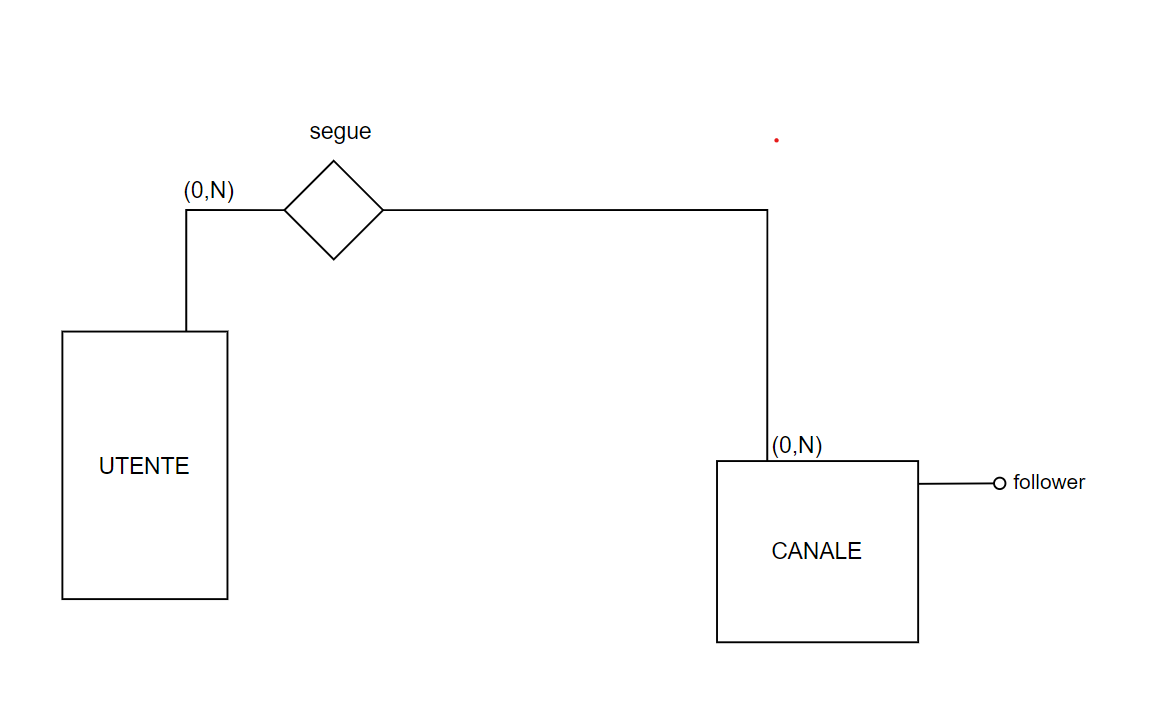
\includegraphics[scale = 0.5]{img/ridondanza1.png}
\end{figure}
\begin{center}
\begin{tabular}{|p{5cm}|p{5cm}|p{5cm}|}
\hline
\multicolumn{3}{|c|}{\textbf{Tavola dei volumi}}\\
\hline
 \multicolumn{1}{|c|}{\textbf{Concetto}} 
 & \multicolumn{1}{|c|}{\textbf{Tipo}}
 & \multicolumn{1}{|c|}{\textbf{Volume}}\\
  \hline
  Utente& E & 5.000.000\\
  \hline
  Canale & E & 5.000.000\\
 \hline 
  Segue & R & 50.000.000\\
 \hline
\end{tabular}
\end{center}
\begin{center}
\begin{tabular}{|p{5cm}|p{5cm}|p{5cm}|}
\hline
\multicolumn{3}{|c|}{\textbf{Tavola delle operazioni}}\\
\hline
 \multicolumn{1}{|c|}{\textbf{Operazone}} 
 & \multicolumn{1}{|c|}{\textbf{Tipo}}
 & \multicolumn{1}{|c|}{\textbf{Frequenza}}\\
  \hline
  Follow di un utente verso un canale & I & 136.986/giorno\\
  \hline
  Calcolo della classifica degli streamer più seguiti & B & 1/settimana\\
 \hline
\end{tabular}
\end{center}


\subsubsection*{Senza ridondanza} 
\textbf{Operazione 1:} Un utente inizia a seguire un altro utente, in media 136.986 volte al giorno.
\begin{figure}[h]
    \centering
    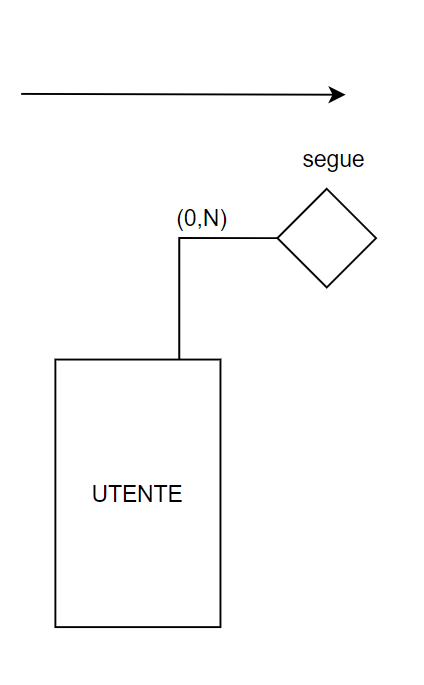
\includegraphics[scale = 0.5]{img/ridondanza11.png}
\end{figure}
\begin{center}
\begin{tabular}{|p{3cm}|p{3cm}|p{3cm}|p{3cm}|}
\hline
\multicolumn{4}{|c|}{\textbf{Tavola degli accessi}}\\
\hline
 \multicolumn{1}{|c|}{\textbf{Concetto}} 
 & \multicolumn{1}{|c|}{\textbf{Costrutto}}
 & \multicolumn{1}{|c|}{\textbf{Accessi}}
 & \multicolumn{1}{|c|}{\textbf{Tipo}}\\
  \hline
  Utente & E & 1 & S\\
  \hline
  Segue & R & 1 & S\\
 \hline
\end{tabular}
\end{center}
\paragraph{Nota Bene} S: Accesso in scrittura. \\ \\
\newpage
\textbf{Operazione 2:} Viene calcolata la classifica dei content creator più seguiti (1 volta a settimana).
\begin{figure}[h]
    \centering
    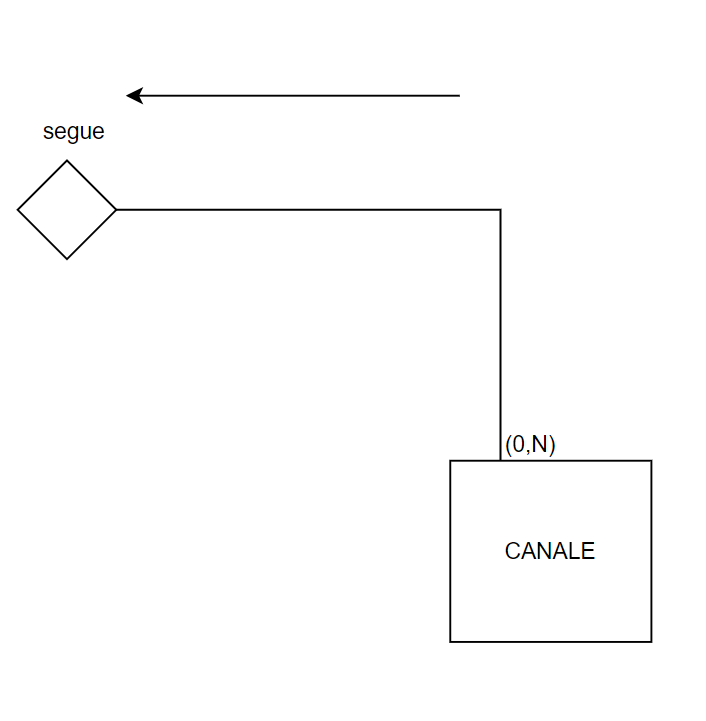
\includegraphics[scale = 0.5]{img/ridondanza111.png}
\end{figure}
\begin{center}
\begin{tabular}{|p{3cm}|p{3cm}|p{3cm}|p{3cm}|}
\hline
\multicolumn{4}{|c|}{\textbf{Tavola degli accessi}}\\
\hline
 \multicolumn{1}{|c|}{\textbf{Concetto}} 
 & \multicolumn{1}{|c|}{\textbf{Costrutto}}
 & \multicolumn{1}{|c|}{\textbf{Accessi}}
 & \multicolumn{1}{|c|}{\textbf{Tipo}}\\
  \hline
  Utente & E & 1 & L\\
  \hline
  Segue & R & 10 & L\\
 \hline
\end{tabular}
\end{center}
Assumendo che, mediamente, un utente segua 10 canali diversi, gli accessi all'associazione sono dati dal seguente calcolo: $(10 \times Volume.Utente) / Volume.Canale = 10$.
\\ \\Analisi dei costi:
\begin{itemize}
    \item Spazio: 0 byte
    \item Tempo:
    \begin{itemize}
        \item Operazione 1: $2 \times (2 \times 958.902)$ accessi in lettura a settimana.
        \item Operazione 2: $10$ accessi in lettura a settimana.
    \end{itemize}
\end{itemize}
Totale: 3.835.618 accessi a settimana.



\newpage
\subsubsection*{Con ridondanza} 
\textbf{Operazione 1:} Un utente inizia a seguire un canale, in media 136.986 volte al giorno.
\begin{figure}[h]
    \centering
    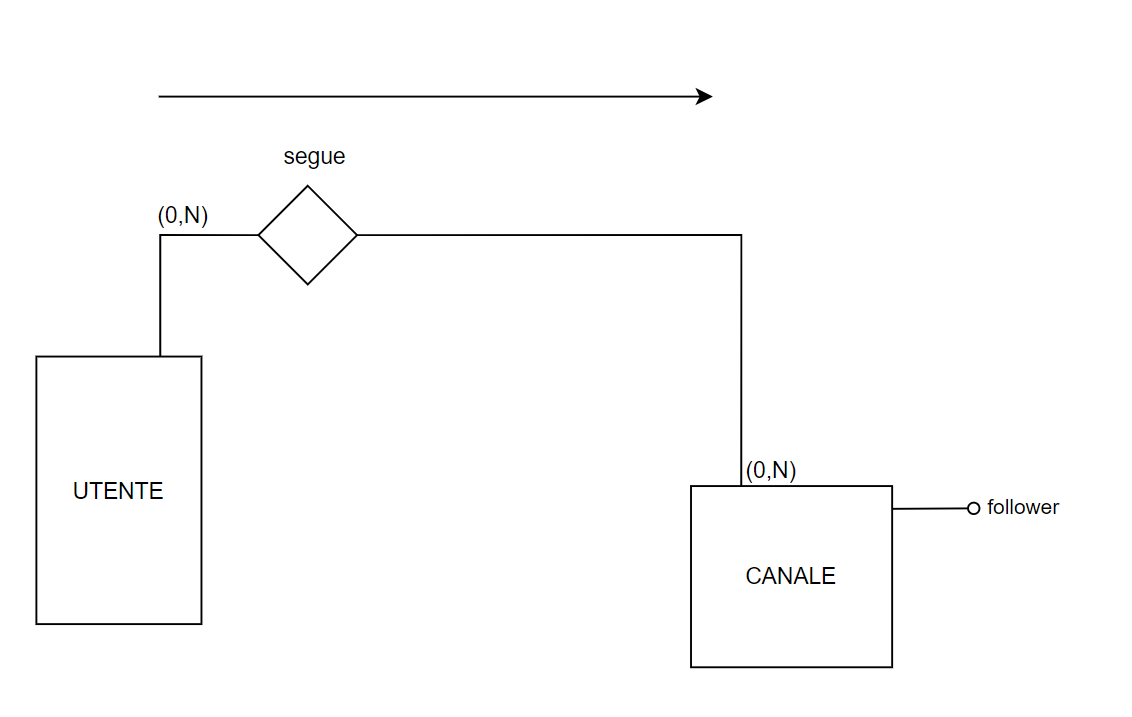
\includegraphics[scale = 0.5]{img/ridondanza2.png}
\end{figure}
\begin{center}
\begin{tabular}{|p{3cm}|p{3cm}|p{3cm}|p{3cm}|}
\hline
\multicolumn{4}{|c|}{\textbf{Tavola degli accessi}}\\
\hline
 \multicolumn{1}{|c|}{\textbf{Concetto}} 
 & \multicolumn{1}{|c|}{\textbf{Costrutto}}
 & \multicolumn{1}{|c|}{\textbf{Accessi}}
 & \multicolumn{1}{|c|}{\textbf{Tipo}}\\
  \hline
  Utente & E & 1 & S\\
  \hline
  Canale & E & 1 & S\\
 \hline
  Segue & R & 1 & S\\
 \hline
\end{tabular}
\end{center}

\textbf{Operazione 2:} Viene calcolata la classifica dei content creator più seguiti (1 volta a settimana).
\begin{figure}[h]
    \centering
    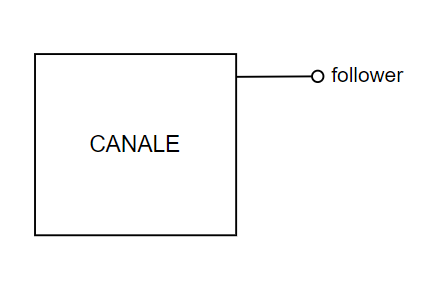
\includegraphics[scale = 0.5]{img/ridondanza22.png}
\end{figure}
\begin{center}
\begin{tabular}{|p{3cm}|p{3cm}|p{3cm}|p{3cm}|}
\hline
\multicolumn{4}{|c|}{\textbf{Tavola degli accessi}}\\
\hline
 \multicolumn{1}{|c|}{\textbf{Concetto}} 
 & \multicolumn{1}{|c|}{\textbf{Costrutto}}
 & \multicolumn{1}{|c|}{\textbf{Accessi}}
 & \multicolumn{1}{|c|}{\textbf{Tipo}}\\
 \hline
  Canale & E & 1 & L\\
 \hline
\end{tabular}
\end{center}
\newpage
Costi:
\begin{itemize}
    \item Spazio: Suppongo di utilizzare 4 byte per il campo \textit{Follower} dell'entità \textit{Canale}, ottengo quindi: 4 byte $\times$ 5.000.000 canali = 20.000.000 byte = 20 MB.
    \item Tempo:
    \begin{itemize}
        \item Operazione 1: $3 \times 958.902$ accessi in scrittura a settimana.
        \item Operazione 2: trascurabile.
    \end{itemize}
\end{itemize}
Totale: 5.753.412 accessi alla settimana

\textbf{Conclusione: } Eliminando la ridondanza diminuisco significativamente non solo il numero di accessi, ma vado anche a risparmiare 20 MB di spazio.








\subsubsection{Eliminazione delle generalizzazioni}
\textbf{Generalizzazione 1:}\\
\begin{figure}[h]
    \centering
    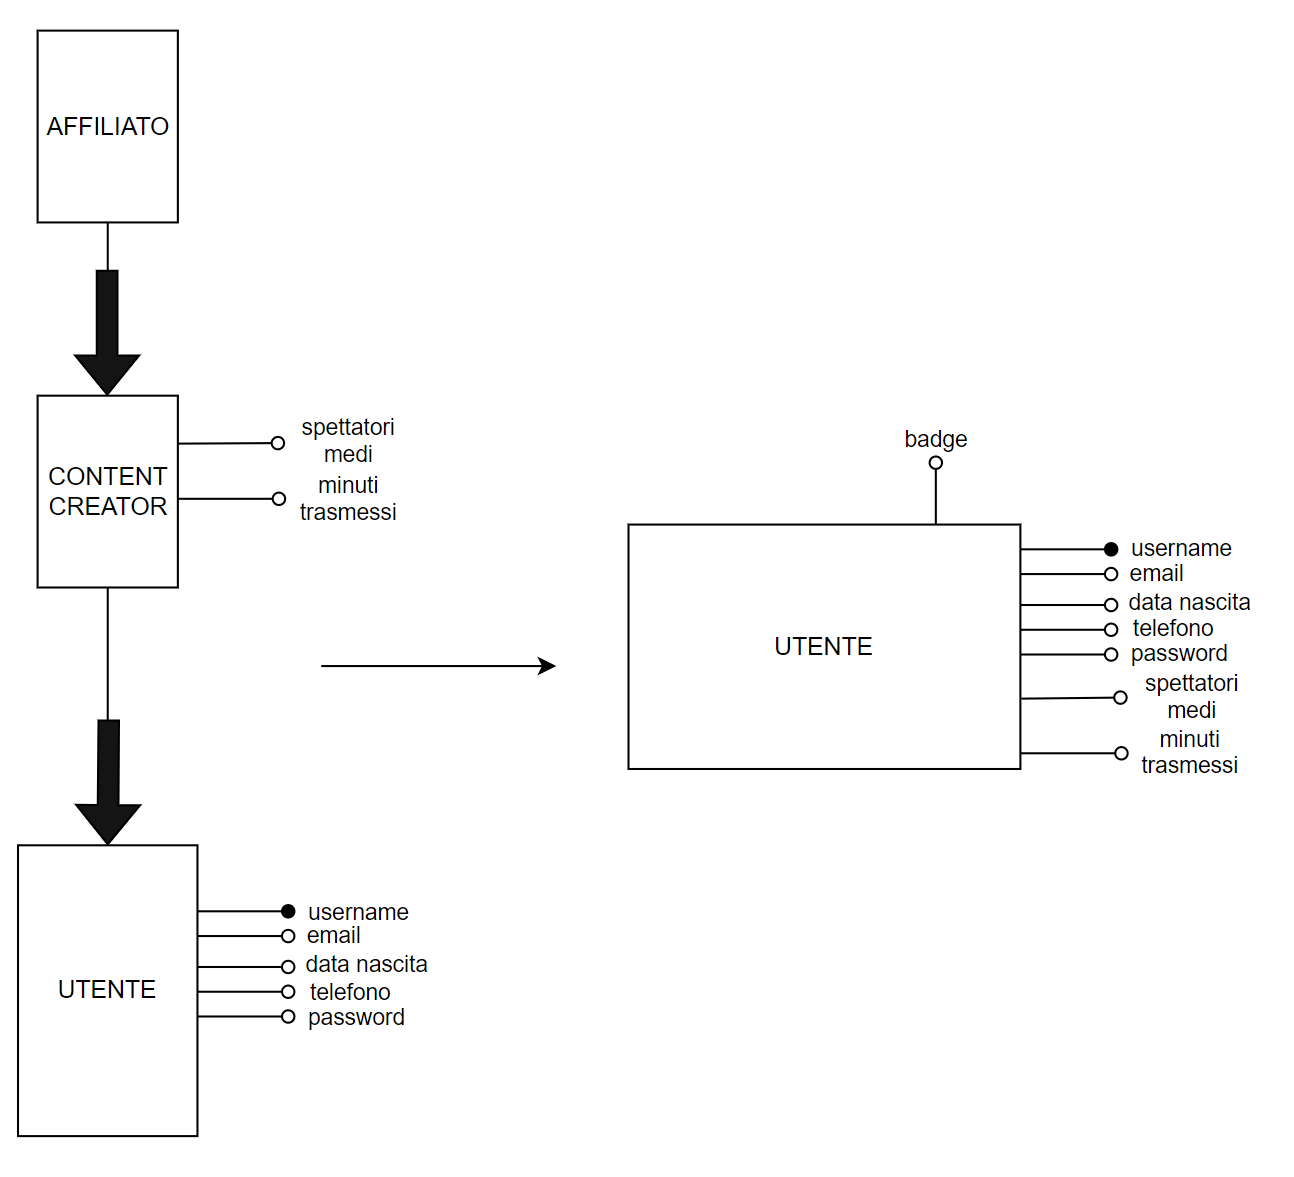
\includegraphics[scale = 0.5]{img/generalizzazione1.png}
\end{figure}\\
\textbf{Business Rules:}
\begin{itemize}
    \item Un \textit{Utente} può diventare \textit{Affiliato} avendo l'attributo booleano \textit{Affiliato} TRUE.
    \item Gli attributi restanti vengono ereditati da \textit{Content Creator} ma possono avere valore 0 nel caso in cui \textit{Utente} decida di non creare alcun contenuto.
\end{itemize}
\textbf{Motivazione:}\\
    L'inclusione delle entità figlie nella loro entità genitore è stata effettuata per ottimizzare lo spazio, mediante la creazione di una nuova tabella che stabilisce una connessione tra \textit{Utente} e \textit{Content Creator}. Questo approccio consente l'ereditarietà degli attributi, come \textit{Minuti trasmessi}, \textit{Spettatori medi} e \textit{Affiliato}, da \textit{Utente}. I primi due sono valori interi e possono rimanere a 0 per gli \textit{Utenti} che non generano contenuti. Nel caso in cui un \textit{Utente}, precedentemente \textit{Content creator}, raggiunga gli obiettivi stabiliti, può acquisire lo status di \textit{Affiliato}. La gestione degli \textit{Affiliati} segue un modello simile su tutte le piattaforme online, consentendo loro di guadagnare un semplice \textit{Affiliato}.


\textbf{Generalizzazione 2:}\\
\begin{figure}[h]
    \centering
    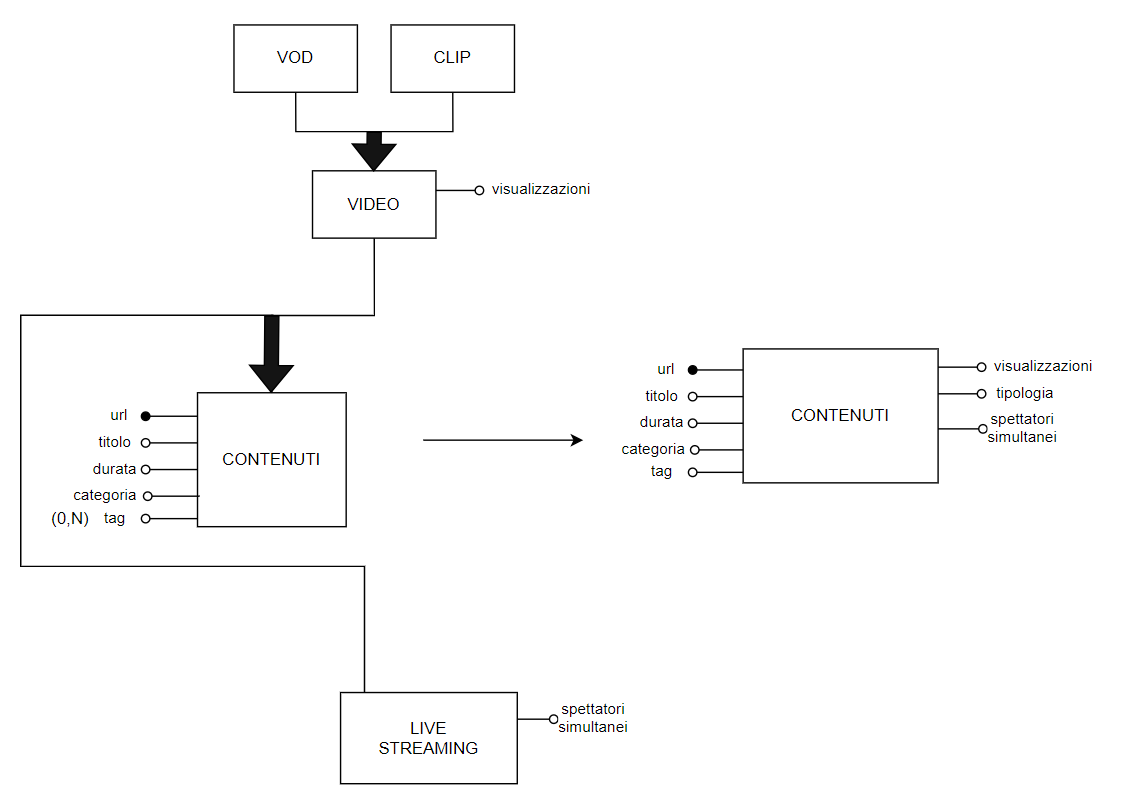
\includegraphics[scale = 0.5]{img/generalizzazione2.png}
\end{figure}\\
\textbf{Business Rules:}
\begin{itemize}
    \item \textit{Tipologia} è un attributo che uso per descrivere le varie istanze delle entità figlie di \textit{Contenuti}.
    \item \textit{Spettatori simultanei} viene utilizzato solamente se \textit{Tipologia} ha valore "Live Streaming".
    \item \textit{Visualizzazioni} viene utilizzato solamente se \textit{Tipologia} ha valore "Video", "Vod" o "Clip".
\end{itemize}
\textbf{Motivazione:}\\
Ho optato per un ulteriore raggruppamento delle entità figlie nella loro entità genitore poiché i \textit{Contenuti} presentano attributi comuni a tutti i figli. Inoltre, considerando che le operazioni non discriminano tra le specializzazioni, la decisione più efficiente è risultata essere l'inclusione dei figli nell'entità genitore. Questa scelta ci ha anche portato a capire che effettuare un raggruppamento del genitore nei figli non sarebbe stata la soluzione ottimale.













\newpage
\subsubsection{Eventuale partizionamento/accorpamento di entità e associazioni}
\textbf{Accorpamento 1:}\\
\begin{figure}[h]
    \centering
    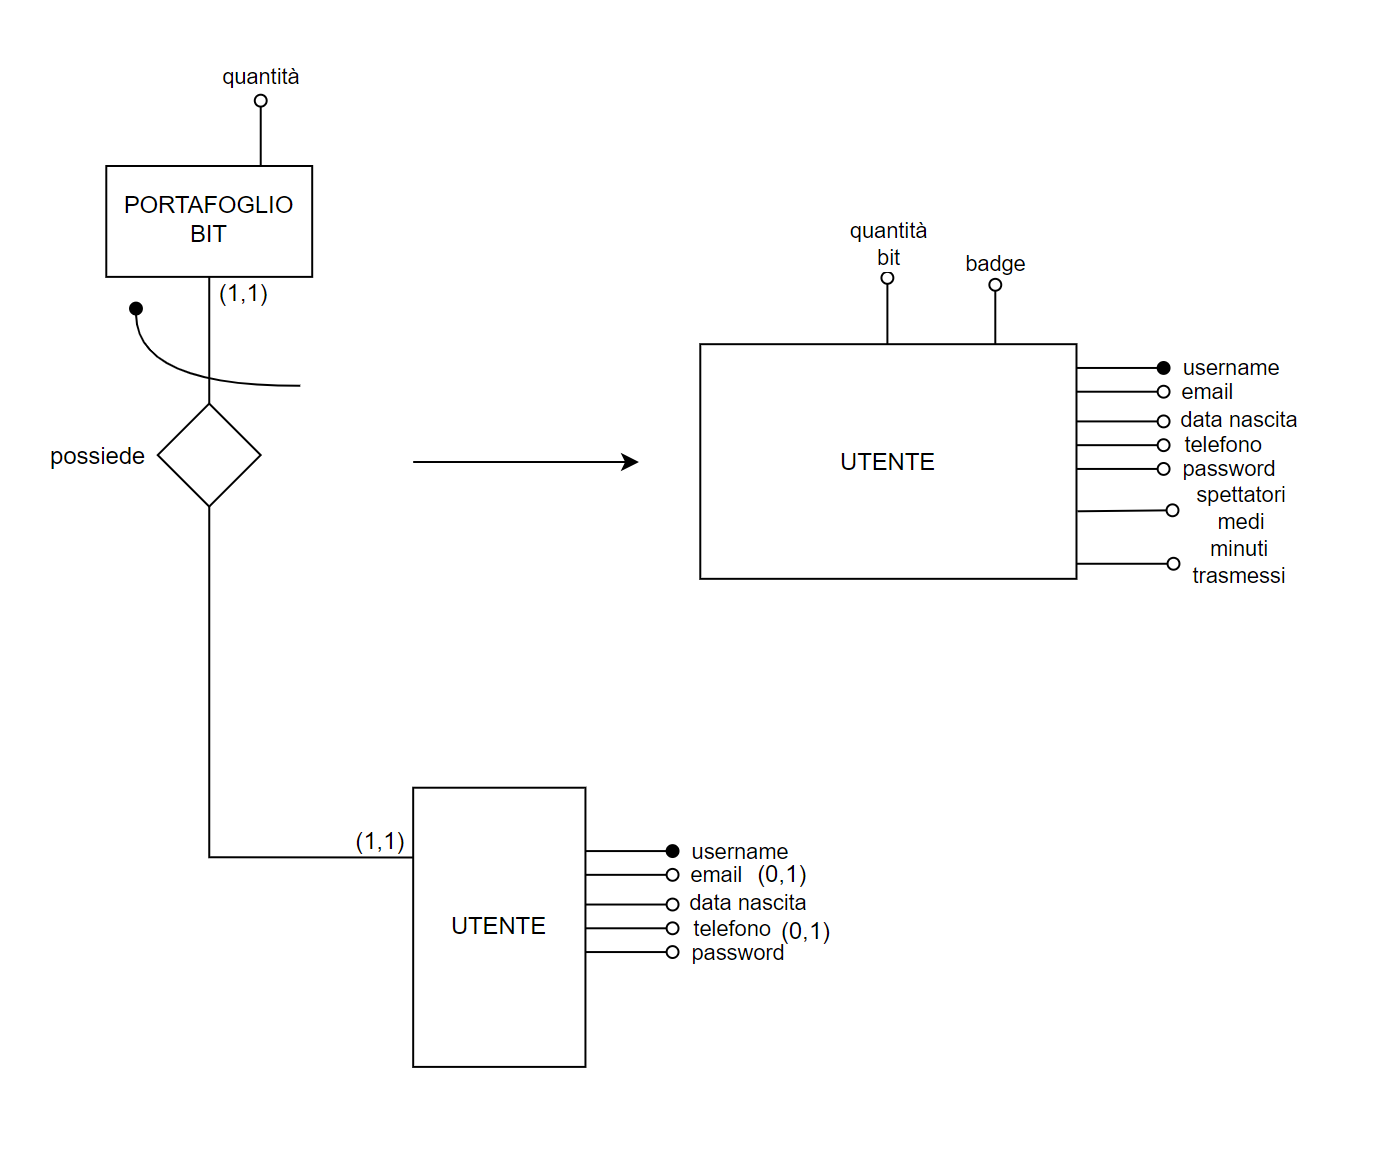
\includegraphics[scale = 0.5]{img/accorpamento1.png}
\end{figure}\\
\textbf{Motivazione:}\\
Ho valutato che le informazioni del \textit{Portafoglio bit} risultano più utili quando sono visualizzate insieme a quelle dell'\textit{Utente}. Considerando il \textit{Portafoglio bit} come un costrutto isolato, offre poche informazioni in quanto richiede sempre lo \textit{Username} per l'accesso. Di conseguenza, poiché ogni \textit{Utente} possiede un unico \textit{Portafoglio bit} e ogni \textit{Portafoglio bit} appartiene a un solo \textit{Utente}, non è necessario creare una nuova tabella per questa entità.



\subsubsection{Eventuale eliminazione delgi attributi composti e degli attributi multivalore}
Gli identificatori principali sono quelli indicati come tali nello schema E-R principale.

\subsubsection{Eventuale scelta degli identificatori principali}
Gli identificatori principali sono quelli indicati come tali nello schema E-R principale.



\newpage
\newgeometry{margin=0.5cm}
\begin{landscape}
\subsection{Schema E-R ristrutturato + business rules}
\vspace{-\parskip} % Elimina lo spazio aggiunto dall'intestazione della subsection
\subsubsection{Schema E-R}
\vspace{-\parskip} % Elimina lo spazio aggiunto dall'intestazione della subsection
\begin{figure}[h]
    \centering
    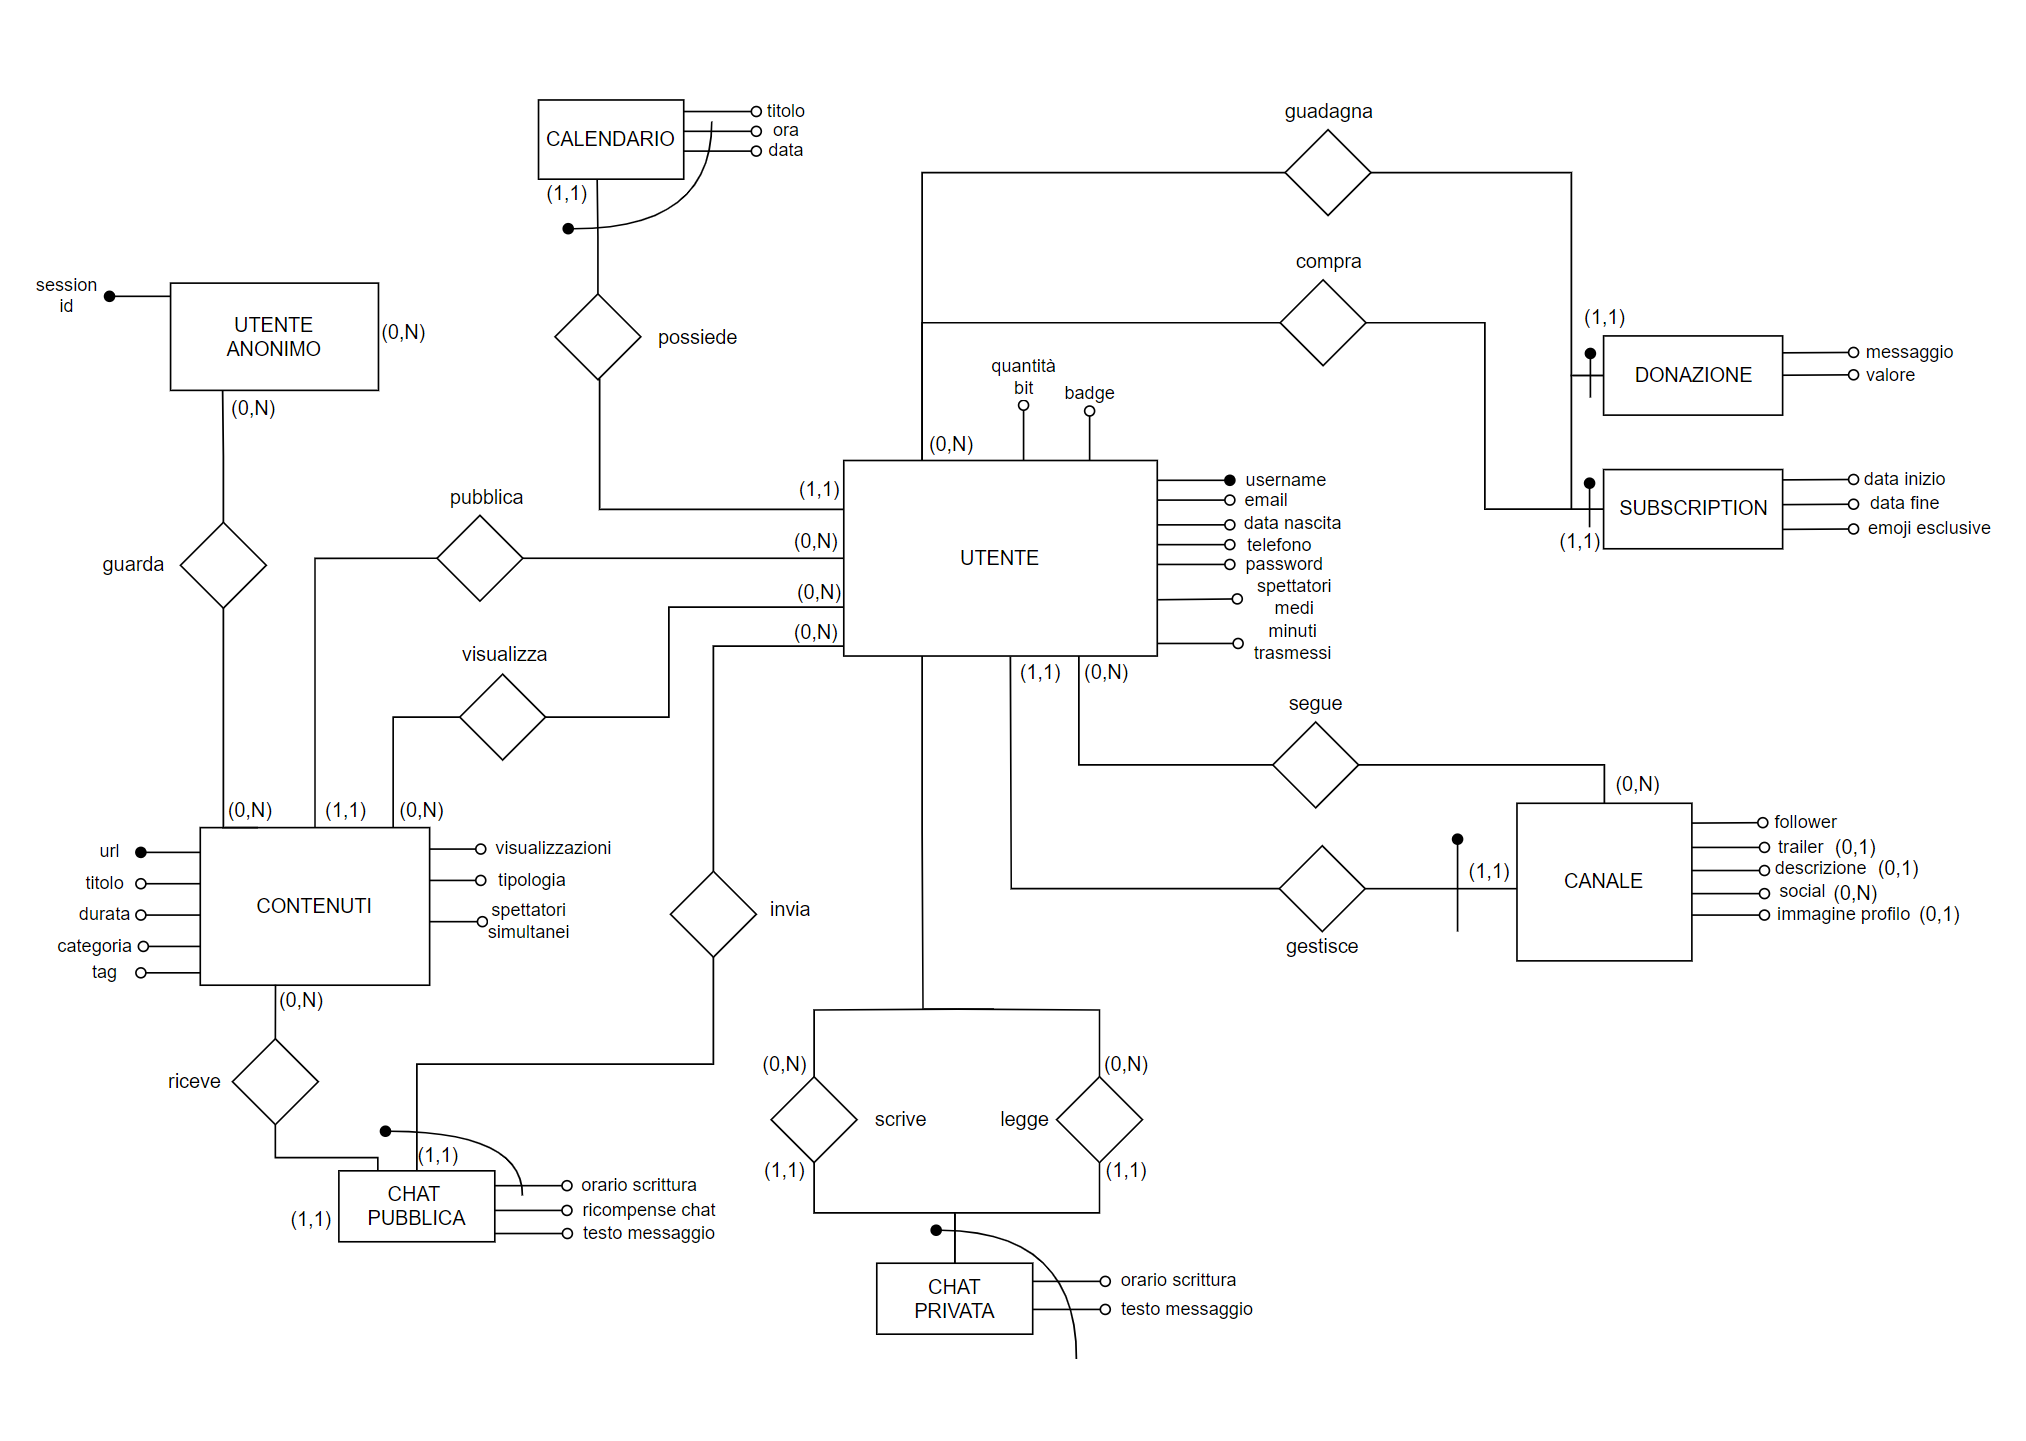
\includegraphics[scale=0.6]{img/ER2.png}
\end{figure}
\end{landscape}
\restoregeometry

%\subsubsection{Business Rules}
%\begin{itemize}
 %   \item Considero gli \textit{Utenti anonimi} come entità separate. Si presume l'esistenza di un algoritmo basato sui log degli utenti non registrati. 
  %  \item Gli \textit{Utenti} devono obbligatoriamente registrarsi sulla piattaforma.
   % \item Gli attributi \textit{Telefono} e \textit{Email} sono stati entrambi impostati come opzionali nello schema E-R poiché per registrarsi alla piattaforma gli utenti devono fornire almeno uno dei due recapiti.
   % \item Il numero di \textit{bit} posseduti da ogni utente deve essere maggiore o uguale a 0.
   % \item Il numero di \textit{bit} donati da un utente a uno streamer deve essere inferiore o uguale al numero di bit posseduti dall'utente in questione.
   % \item I due \textit{Utenti} coinvolti in una\textit{Chat privata} non possono essere lo stesso utente, poiché risulta ovviamente incoerente che un utente invii messaggi a se stesso.
%\end{itemize}










































\subsection{Schema relazionale}
\begin{itemize}
    \item \textbf{Utente} (\underline{username}, email*, telefono*, dataNascita, password, spettatoriMedi, minutiTrasmessi, quantitàBit, affiliato)
    \item \textbf{Calendario} (\underline{username, data, ora}, titolo)
    \item \textbf{UtenteAnonimo} (\underline{sessionId})
    \item \textbf{Contenuti} (\underline{url}, nomeContentCreator, titolo, durata, categoria, tag, visualizzazioni, tipologia, spettatoriSimultanei)
    \item \textbf{ChatPubblica} (\underline{orarioScrittura, utenteMittente, url}, ricompenseChat, testoMessaggio)
    \item \textbf{ChatPrivata} (\underline{orarioScrittura, testoMessaggio, utenteMittente, utenteDestinatario})
    \item \textbf{Canale} (\underline{username}, follower, trailer*, descrizione*, immagineProfilo*, social)
    \item \textbf{Subscription} (\underline{subber, subbed}, dataInizio, dataFine, emojiEsclusive)
    \item \textbf{Donazione} (\underline{donatore, beneficiario}, messaggio, valore)
    \item \textbf{Guarda} (\underline{sessionID, url})
    \item \textbf{Segue} (\underline{seguace}, \underline{seguito})
    \item \textbf{Visualizza} (\underline{url, username})
\end{itemize}

\subsubsection*{Vincoli di integrità referenziale}
\begin{itemize}
  \item \textbf{Calendario} (\textit{username}) referenzia \textbf{Utente} (\textit{username})
  \item \textbf{chatPubblica} (\textit{utenteMittente}) referenzia \textbf{Utente} (\textit{username})
  \item \textbf{chatPubblica} (\textit{url}) referenzia \textbf{Contenuti} (\textit{url}) 
  \item \textbf{chatPrivata} (\textit{utenteMittente}) referenzia \textbf{Utente} (\textit{username})
  \item \textbf{chatPrivata} (\textit{utenteDestinatario}) referenzia \textbf{Utente} (\textit{username})
  \item \textbf{Canale} (\textit{username}) referenzia \textbf{Utente} (\textit{username})
  \item \textbf{Subscription} (\textit{subber}) referenzia \textbf{Utente} (\textit{username})
  \item \textbf{Subscription} (\textit{subbed}) referenzia \textbf{Utente} (\textit{username})
  \item \textbf{Donazione} (\textit{donatore}) referenzia \textbf{Utente} (\textit{username})
  \item \textbf{Donazione} (\textit{beneficiario}) referenzia \textbf{Utente} (\textit{username})
  \item \textbf{Guarda} (\textit{sessionId}) referenzia \textbf{UtenteAnonimo} (\textit{sessionID})
  \item \textbf{Guarda} (\textit{url}) referenzia \textbf{Contenuti} (\textit{url})
  \item \textbf{Segue} (\textit{seguace}) referenzia \textbf{Utente} (\textit{username})
  \item \textbf{Segue} (\textit{seguito}) referenzia \textbf{Utente} (\textit{username})
  \item \textbf{Visualizza} (\textit{url}) referenzia \textbf{Contenuti} (\textit{url})
  \item \textbf{Visualizza} (\textit{username}) referenzia \textbf{Utente} (\textit{username})
\end{itemize}
